\chapter[Strucuture of Crystals and Liquids]{Ground State Structures of Molecular Crystals and Liquids}
\label{sec:structure}

As we lower the temperature, the properties of the condensed phase become increasingly dominated by the arrangement of molecules corresponding to the local potential energy minima, the ground state. This is similar to the way that the structure and dynamics of a small molecule can be inferred from its ground state structure. In the same way these properties can be inferred from the ground state structure of these condensed phases containing thousands of molecules.

In this chapter we address a number of structural properties of our molecules. In \textsecref{crys phase} we find the most stable crystal phase for our molecules. In \textsecref{order parameter} we develop methods to identify order including whether it is possible to identify order in all crystal structures with a single measure of order. In \textsecref{order inherent} we use the order parameters to investigate order in the ground state structures of the supercooled liquid configurations from \textchapref{dynamics}.

\section{The Most Stable Crystal Phase}
\label{sec:crys phase}

The most stable crystal phase, for our purposes, is the crystal that will form spontaneously from the liquid phase upon cooling. Since by design this process is slow or unobservable for the molecular liquids we are using we need to use other means to identify the most stable crystal phase (described below). Of most stable crystal phases~\figref{crystals} the \dcon and \tri molecules have unit cells in the p2 wallpaper group \appref{wallpaper} which contains the majority of crystals~\cite{plass:07,jennings:15}. The \done molecule has a stable crystal with the p2mg wallpaper group, a wallpaper group which contains very few crystal structures, making the crystal structure inherently interesting. It should be noted that all the crystal structures contain molecules paired the maximum number of interactions and an inversion center between them. It is likely that the formation of this interlocking structure plays a role in stabilising these crystal phases.

\begin{figure}
    \centering
    \begin{subfigure}[t]{0.45\linewidth}
        \includegraphics[width=\textwidth]{{{Snowman-0.4-0.637556-1.00-p2mg-frame}}}
        \caption{}
        \label{fig:crystal done}
    \end{subfigure}\hfill
    \begin{subfigure}[t]{0.45\linewidth}%
        \includegraphics[width=\textwidth]{{{Snowman-0.4-0.637556-1.637556-p2-frame}}}
        \caption{}
        \label{fig:crystal dcon}
    \end{subfigure}
    \begin{subfigure}{0.45\linewidth}
        \includegraphics[width=\textwidth]{{{Trimer-0.4-0.637556-1.00-120-p2-frame}}}
        \caption{}
        \label{fig:crystal tri}
    \end{subfigure}
    \caption{The stable crystal forms of the \done p2mg~\subfigref{crystal done}, \dcon p2~\subfigref{crystal dcon}, and \tri p2~\subfigref{crystal tri} molecules. The molecules are coloured according to their orientation. The unit cell is indicated by a black box with an inversion center marked with a red dot.}
    \label{fig:crystals}
\end{figure}

The crystal structures shown in \textfigref{crystals} were determined to be the most stable crystal structures using a variety of techniques. As a starting point we wanted to find the lowest energy crystal structures, since using molecular dynamics was not possible we had to use an alternate method. By approximating our particles as hard discs and finding the closest packed structure we are able to use the isopointal search algorithm developed by~\textcite{hudson:10} to search the reduced packing space, generating a series of best packed structures.

The best packed structures were then used as the starting configurations for a molecular dynamics simulation to find the lowest energy ground state~\tabref{crystal energies}. The \done and \dcon molecules have configurations with a ground state significantly lower than any other, p2mg and p2 respectively. For these two molecules we can be fairly certain these are the most stable ground state, however for the \tri molecule there are three configurations p2, p2gg and pg all with similar ground state energies.

\begin{table}
    \sisetup{
        table-format = +3.4,
        table-omit-exponent,
        fixed-exponent =-4,
        parse-numbers=true,
        scientific-notation=true,
        round-mode=places,
        round-precision=3}
    \centering
    \begin{tabular}{ | l | S  S  S | }
        \hline
        {Crystal} & \multicolumn{3}{c|}{Energy per molecule (\num{e-4})} \\
            &\done & \dcon & \tri \\ \hline
        p2 & 0.00001376280055& {\cellcolor{blue!20}}0.0001527208398& {\cellcolor{blue!10}}-0.0003934685913\\
        p2mg & {\cellcolor{blue!20}}0.000005732595806& 0.0004479052484& -0.0003354198174\\
        p2gg & 0.00002632511042& 0.0001699363766& {\cellcolor{blue!20}}-0.000401823091\\
        pg & 0.00002824743917& 0.0002860863393& {\cellcolor{blue!10}}-0.0004000561542\\
        p3 & 0.00003468842645& 0.0002424453316& -0.0003292839541\\
        \hline
    \end{tabular}
    \caption{The ground state energy per molecule for a variety of the best packing initial configurations, the lowest energies are shaded blue. Both the \done and \dcon systems have an arrangement with significantly lower energy, p2mg and p2 respectively. In contrast the \tri system has three arrangements with very similar energies, the p2, p2gg and pg wallpaper groups.}
    \label{tab:crystal energies}
\end{table}

With multiple structures of the \tri molecule having similar ground state energies further analysis is required to determine the most stable structure, for this we looked to a two phase system as described in \textsecref{two phase}. The two phase system~\figref{tri two phase} showed a solid state rearrangement of molecules from the p2gg structure, which had the lowest ground state energy, to the p2 structure. One possible reason for this rearrangement is the p2 structure allows more vibrational motion at higher temperatures providing an entropic stabilisation of this structure.

\begin{figure}
    \begin{subfigure}[t]{0.5\textwidth}
        \includegraphics[width=\textwidth]{{{Trimer-1.30-0.637556-1.00-120-p2gg-1-frame-0000000000}}}
        \caption{Initial}
        \label{fig:tri rearr init}
    \end{subfigure}
    \begin{subfigure}[t]{0.5\textwidth}
        \includegraphics[width=\textwidth]{{{Trimer-1.30-0.637556-1.00-120-p2gg-1-frame-0320000000}}}
        \caption{Final}
        \label{fig:tri rearr fine}
    \end{subfigure}
    \caption{The initial~\subfigref{tri rearr init} and final~\subfigref{tri rearr fine} configurations of a two phase crystal-liquid simulation of the \tri molecule below the melting point. We can see the solid state phase transition from a p2mg structure with four layers in each unit cell to a structure that alternates between the p2 structure (two layers) and the p2gg structure (four layers).}
    \label{fig:tri two phase}
\end{figure}

In light of the \tri molecule having a stable structure that is not the lowest energy ground state we performed melting point analysis on both the \done and \dcon molecules. The melting points~\tabref{melting} for each crystal were obtained using a two phase crystal-liquid system (see \textsecref{two phase} for details). These results confirmed the lowest energy structures were the most stable having significantly higher melting points than the other structures.

\begin{table}
    \centering
    \begin{tabular}{| l l | S |}
        \hline
        Molecule & Crystal & {Melting Point} \\ \hline
        \multirow{3}{*}{\done} & p2 & 0.65 \\
                               & p2gg & 0.55 \\
                               & p2mg & 0.92 \\ \hline
        \multirow{2}{*}{\dcon} & p2 & 1.85 \\
                               & p2gg & 1.50 \\ \hline
    \end{tabular}
    \caption{Melting points of the crystal phases established from two phase crystal-liquid systems (see \textsecref{two phase} for details).}
    \label{tab:melting}
\end{table}

\section{Quantifying Order in Molecular Systems}
\label{sec:order parameter}

In most cases it is fairly easy to distinguish a crystal from an amorphous phase by simple visual inspection of the two configurations. Much harder to determine visually is to quantify the degree to which a system is ordered, a problem with application in crystal growth. In this section we investigate a number of measures of order, including local order, as well as problems associated with each. We will be investigating these order parameters using an amorphous ground state from the supercooled \dcon liquid in \textchapref{dynamics} and the most stable ground state crystal configuration~\figref{frame comp} of the \dcon molecule.

\begin{figure}
    \begin{subfigure}{0.5\textwidth}
        \includegraphics[width=\linewidth]{amorphous-frame}
        \caption{}
        \label{fig:amorphous frame}
    \end{subfigure}
    \begin{subfigure}{0.5\textwidth}
        \includegraphics[width=\linewidth]{crys-frame}
        \caption{}
        \label{fig:crys frame}
    \end{subfigure}
    \caption{The amorphous ground state\subfigref{amorphous frame} and most stable crystal \subfigref{crys frame} configurations of the \dcon molecule with the colour of the molecules indicating orientation.}
    \label{fig:frame comp}
\end{figure}

The first of the order parameters is the radial distribution function~\figref{radial comp}, a distribution of the relative intermolecular distances. The amorphous structure shows short range ordering characteristic of any condensed phase, however this order is only present in the first layer and second shell of neighbours, once past this region ($r>4$) the distribution of molecules is uniform. This is in contrast with the crystal structure that exhibits distinct peaks out to the edge of the plot showing long range order.

\begin{figure}
    \begin{subfigure}{0.5\textwidth}
        \includegraphics[width=\linewidth]{amorphous-radial}
        \caption{}
        \label{fig:amorphous radial}
    \end{subfigure}
    \begin{subfigure}{0.5\textwidth}
        \includegraphics[width=\linewidth]{crys-radial}
        \caption{}
        \label{fig:crys radial}
    \end{subfigure}
    \caption{The radial distribution function of the amorphous ground state \subfigref{amorphous radial} and most stable ground state crystal \subfigref{crys radial} configurations. The amorphous structure shows a peak at short range which quickly becomes a uniform distribution. The crystal structure shows sharp peaks out to long ranges.}
    \label{fig:radial comp}
\end{figure}

Along with the global order measured by the radial distribution function we can also measure local order to classify individual molecules as crystalline or amorphous. This allows us to count the number of molecules that are considered crystalline, an easy measure of crystal growth. The crystal structures of all three molecules have the molecules aligned antiparallel to each other, molecules are aligned either \ang{0} or \ang{180} relative to each other. We can use this local orientational order to define a local order parameter $O_\text{orient}$,
\begin{equation}
    O_{\text{orient}} = \frac{1}{N_{\text{neigh}}}\sum_{i=1}^{N_\text{neigh}} (\vect{\hat e} \cdot \vect{\hat e_i})^2
\end{equation}
where $N_\text{neigh}$ is the number of neighbours, $\vect{\hat e}$ is the unit orientation vector of the molecule and $\vect{\hat e_i}$ is the unit orientation vector of each neighbour. In the perfect ground state crystal structure molecules with $O_\text{orient}=1$ would be considered crystalline, however to account for the rotations and vibrations of molecules when heated above the ground state a cutoff of \num{0.8} was chosen as being best at differentiating crystal $O_\text{orient}> 0.8$ and amorphous $O_\text{orient} < 0.8$ regions. To assist in identifying this local order within a configuration~\figref{orient comp} we can colour the ordered molecules leaving all others grey. Since this local order parameter identifies molecules with antiparallel orientations the molecules are coloured such that both have the same colour showing the orientation of the resulting crystal. The coloured regions of the amorphous phase show molecules or small clusters that exhibit short range ordering, because of the number of local orderings in the amorphous phase some are going to be considered locally crystalline.

\begin{figure}
    \begin{subfigure}{0.5\textwidth}
        \includegraphics[width=\linewidth]{amorphous-local}
        \caption{}
        \label{fig:amorphous local}
    \end{subfigure}
    \begin{subfigure}{0.5\textwidth}
        \includegraphics[width=\linewidth]{crys-local}
        \caption{}
        \label{fig:crys local}
    \end{subfigure}
    \caption{Ground state configurations of the amorphous \subfigref{amorphous local} and crystal \subfigref{crys local} configurations identifying local orientational order $O_\text{orient}$. The molecules are coloured according to the orientation of the crystal. The crystal phase shows a single purple crystal for the entire configuration, while the amorphous phase contains a few individual molecules showing local crystalline order at different orientations.}
    \label{fig:orient comp}
\end{figure}

\subsection{Problems with Generic Descriptions of Order in Molecular Systems}

The \dcon molecule was chosen for being a special case, this ratio of hard discs will form a compact packing~\appref{compact}. If we start with the compact packing of discs~\figref{compact} we can assign bonds between large and small particles to form \dcon molecules without modifying the underlying structure. Two examples of this assignment of bonds, an orientationally ordered p2 structure~\figref{ordered frame} and an orientationally disordered random assignment of bonds~\figref{random frame}. Both these structures have the same underlying structure of particles, despite the orientational disorder in the randomly assigned configuration it is indisputably crystalline in character and any order parameter should reflect this.

\begin{figure}
    \centering
    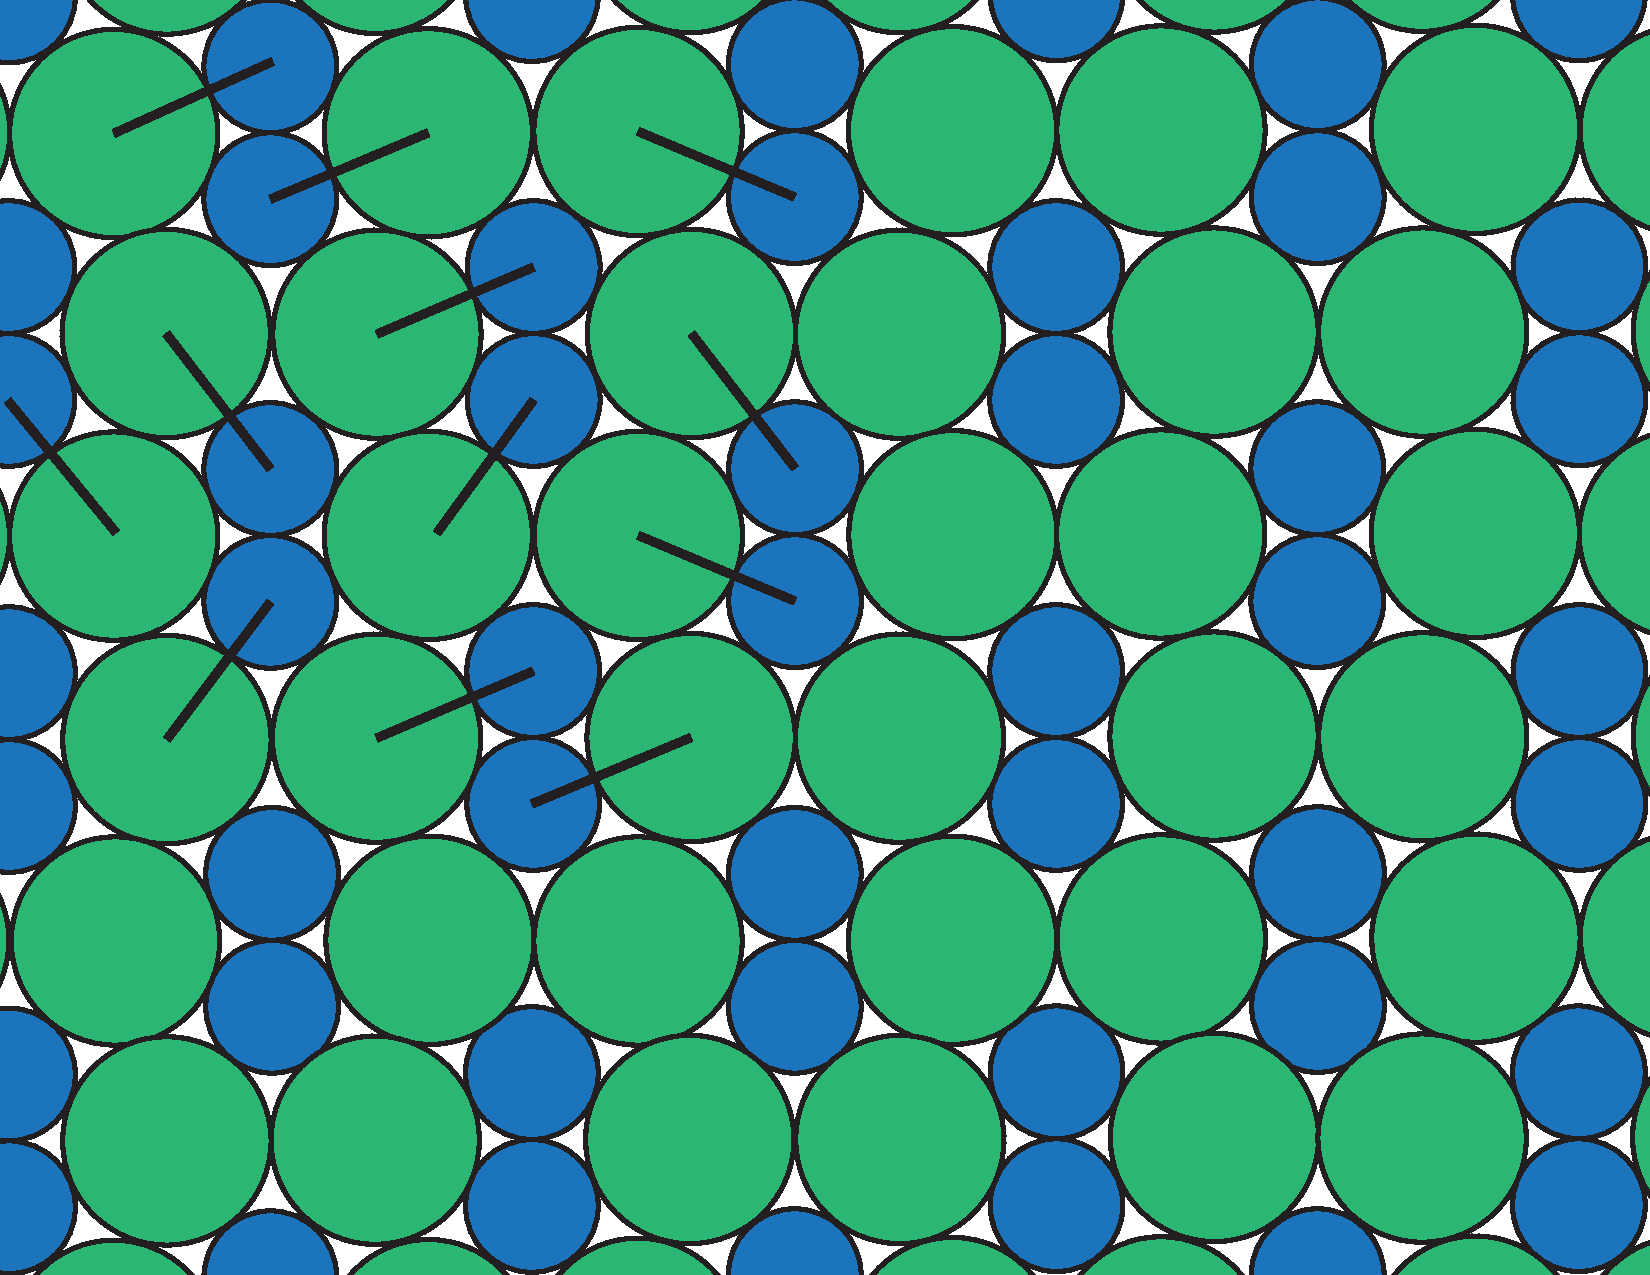
\includegraphics[width=0.5\textwidth]{compact}
    \caption{The compact packing of discs with ratio 1:0.637556. Assignment of bonds to this structure can be performed randomly (top left) with no alteration of the underlying structure.}
    \label{fig:compact}
\end{figure}

Using the local order parameter~\figref{compact local} the orientationally ordered configuration has the expected crystal structure while the orientationally disordered structure is not considered crystalline. For the \dcon molecule the more complex and specific crystal phase makes a general order parameter insufficient to resolve the crystal structure. Instead we want a local order parameter designed specifically for the \dcon system.

\begin{figure}
    \begin{subfigure}[t]{0.5\linewidth}
        \includegraphics[width=\linewidth]{random-local}
        \caption{}
        \label{fig:random local}
    \end{subfigure}
    \begin{subfigure}[t]{0.5\linewidth}
        \includegraphics[width=\linewidth]{ordered-local}
        \caption{}
        \label{fig:ordered local}
    \end{subfigure}
    \caption{Comparison of the local orientation order parameter $O_\text{orient}$ on the randomly oriented \subfigref{random local} and orientationally ordered \subfigref{ordered local} crystalline configurations of the \dcon molecule.}
    \label{fig:compact local}
\end{figure}

The crystalline structure of the \dcon molecule is defined by the underlying arrangement of particles, the arrangement of bonds on top of the arrangement of particles does not contribute to the crystal structure. As such we want an order parameter $O_\dcon$ based on the arrangement of individual particles rather than molecules. The way we have done this is to consider the local environment of each particle. In the crystalline structure each small particle has one small and four large neighbouring particles, and each large particle has three small and three large neighbours. By counting the number and type of neighbours particles with the appropriate local environment are classed as crystalline. 

While in these ground state configurations we see the molecules touching once heated up these contacts disappear. In these higher temperature cases we need a more robust definition of neighbour. We have defined two particles as being neighbouring if they are within a distance of $1.2(r_1 +r_2)$ where $r_1$ and $r_2$ are the radii of the two molecules and the factor of 1.2 is chosen to include all the first shell neighbours in the liquid phase.

Using this targeted order parameter~\figref{compact frame} both the structures with random orientation and ordered orientation are completely crystalline. This demonstrates that the order parameters need to be carefully matched with the molecule to accurately identify the crystal phase.

\begin{figure}
    \begin{subfigure}[t]{0.5\linewidth}
        \includegraphics[width=\linewidth]{random-frame}
        \caption{}
        \label{fig:random frame}
    \end{subfigure}
    \begin{subfigure}[t]{0.5\linewidth}
        \includegraphics[width=\linewidth]{ordered-frame}
        \caption{}
        \label{fig:ordered frame}
    \end{subfigure}
    \caption{Comparison of the $O_\dcon$ order parameter on the randomly oriented \subfigref{ordered frame} and orientationally ordered \figref{random frame} crystal configurations of the \dcon molecule. All molecules are considered crystalline and coloured according to their orientation.}
    \label{fig:compact frame}
\end{figure}

\section{The Structure in Amorphous Ground States}
\label{sec:order inherent}

While liquids show no long range anisotropy there is no reason why they might not accumulate short range structure as they are cooled below their freezing point. By \emph{short range} or \emph{local} structure we are referring to small clusters of particles that adopt an ordered arrangement that does not extend beyond the cluster. Using the tools developed above, in this section we investigate local structure of the supercooled liquid state using their ground state configurations.

The \done molecule~\figref{done order} shows a small degree of long range ordering of the ground state in the radial distribution function, which we can see as mostly small clusters of local crystalline order, with some larger crystals in the local order parameter \oorient. These larger crystals are the crystal phase nucleating and their presence in the ground state structure suggests that it will be possible to grow crystals of the \done molecule in \textchapref{crystallisation}.

\begin{figure}
    \centering
    \begin{subfigure}[t]{0.45\linewidth}
        \includegraphics[width=\linewidth]{{{Snowman-0.80-0.637556-1.0-radial}}}
        \caption{}
        \label{fig:done radial}
    \end{subfigure}\hfill
    \begin{subfigure}[t]{0.45\linewidth}
        \includegraphics[width=\textwidth]{{{Snowman-0.80-0.637556-1.0-frame-0320000191}}}
        \caption{}
        \label{fig:done inherent}
    \end{subfigure}\hfill
    \caption{Ground state radial distribution function \subfigref{done radial} and local ordering \oorient \subfigref{done inherent} of the \done molecule. The broad peaks of the radial distribution function out a distance of 12 indicate some longer range ordering present in the structure, which we see in the configuration as small clusters of local crystalline ordering. The large cluster shows a nucleation event, demonstrating that crystal nucleation is possible.}
    \label{fig:done order}
\end{figure}

The ground state of the \dcon molecule appears to be amorphous from the radial distribution function~\figref{dcon inherent} however the local order parameter \ocon shows regions of orientationally disordered crystalline order. In developing the local order parameter \ocon for \dcon we used the local order of the particles as a measure of the local order of the molecules, we can define a radial distribution function in the same way such that we are looking at the distances between each particle rather than each center of mass. This alternate radial distribution function gives \textfigref{dcon radial part} which shows medium range ordering like we observe with the local order parameter \ocon.

\begin{figure}
    \centering
    \begin{subfigure}[t]{0.5\linewidth}
        \includegraphics[width=\linewidth]{{{Snowman-1.55-0.637556-1.637556-radial}}}
        \caption{}
        \label{fig:dcon radial}
    \end{subfigure}\hfill
    \begin{subfigure}[t]{0.5\linewidth}
        \includegraphics[width=\textwidth]{{{Snowman-1.55-0.637556-1.637556-frame-0320000182}}}
        \caption{}
        \label{fig:dcon inherent}
    \end{subfigure}
    \caption{Ground state radial distribution function \subfigref{dcon radial} and local order parameter \ocon \subfigref{dcon inherent} of the \dcon molecule. The initial peaks of the radial distribution function are sharp showing strong short range ordering, however this order only extends to the second coordination shell. The local order parameter reveals clusters of orientationally disorderd crystalline clusters.}
        \label{fig:dcon order}
\end{figure}

\begin{figure}
    \centering
    \includegraphics[width=0.5\linewidth]{{{Snowman-1.55-0.637556-1.637556-radial_part}}}
    \caption{Interparticle radial distribution function for particles in the ground state configuration of the \dcon molecule. This is a distribution of interparticle distances rather than center of mass distances. This figure reveals the presence of medium-range ordering that extends out to a distance of 12.}
    \label{fig:dcon radial part}
\end{figure}

The \tri molecule shows no ordering in the ground state configuration~\figref{tri order} from either the radial distribution function or the local order parameter \oorient. While there are some regions of local orientational order indicated by coloured molecules, these are a combination of the molecules occupying all the possible arrangements and false positives. From inspection of the configuration the regions of local order identified are not representative of any longer range order. This lack of order is intriguing since ground state of the \tri molecule was found further below the melting point than either of the other molecules with no indication of any order. It is a truly amorphous phase.

\begin{figure}
    \begin{subfigure}{0.5\linewidth}
        \includegraphics[width=\linewidth]{{{Trimer-1.05-0.637556-1.00-120-radial}}}
        \caption{}
        \label{fig:tri radial}
    \end{subfigure}
    \label{fig:radial distributions}
    \begin{subfigure}{0.5\linewidth}
        \includegraphics[width=\textwidth]{{{Trimer-1.00-0.637556-1.00-120-frame-0320000177}}}
        \caption{}
        \label{fig:tri inherent}
    \end{subfigure}
    \caption{Ground state radial distribution function \subfigref{tri radial} and local order parameter \oorient \subfigref{tri inherent} of the \tri molecule. Neither the radial distribution function or the local order parameter display any signs of medium range ordering.}
    \label{fig:tri order}
\end{figure}

\section{Summary}

In this Chapter we have identified the most stable crystal forms of each of our molecules as well as order parameters enabling us to distinguish the amorphous liquid phase from the ordered crystal phase. In investigating ordering of the \dcon molecule we discovered that using a single order parameter for all molecules is inadequate and that the order parameters need to be tuned for each system. The order parameters we have identified will allow us to investigate the growth of the crystal from the liquid phase, which is the focus of the next Chapter.
